\documentclass{article}
\usepackage{etoolbox}
\usepackage{qrcode}
\usepackage{geometry}
\geometry{a0paper,margin=1cm}
\usepackage{graphicx}
\usepackage{enumitem}
\setlist{leftmargin=*,nosep,noitemsep}
\usepackage{anyfontsize}
\usepackage[sfdefault]{roboto}
\usepackage[T1]{fontenc}
\usepackage{tikz}
\pagestyle{empty}
\usepackage{siunitx}
\usepackage{booktabs}
\sisetup{
        % detect-all,
        mode = match ,
        propagate-math-font = true ,
        reset-math-version = false ,
        reset-text-family = false ,
        reset-text-series = false ,
        text-family-to-math = true ,
        text-series-to-math = true ,
        range-phrase=\,--\,,
        group-separator={,},
        group-minimum-digits=3,
        group-digits=integer,
    }
\usepackage{caption}
\DeclareCaptionFormat{paper}{\fontsize{20pt}{25pt}\selectfont#1#2#3}
\captionsetup{format=paper}
\usepackage{xurl}
\usepackage{hyperref}
\urlstyle{same}
% Title, authors, affiliations
    \newcommand{\dbtitle}{}        \renewcommand{\title}[1]{\renewcommand{\dbtitle}{#1}}
    \newcommand{\dbauthors}{}      \newcommand{\authors}[1]{\renewcommand{\dbauthors}{#1}}
    \newcommand{\dbaffiliations}{} \newcommand{\affiliations}[1]{\renewcommand{\dbaffiliations}{#1}}
    \newcommand{\dbQRcode}{} \newcommand{\QRcode}[1]{\renewcommand{\dbQRcode}{#1}}
%
    \usepackage[table]{xcolor}
    \definecolor{lightblue}{RGB}{189,215,238}
    \definecolor{medblue}{RGB}{141,180,226}
    \definecolor{darkblue}{RGB}{46,117,182}
    \definecolor{lightorange}{RGB}{248,203,173}
    \definecolor{medorange}{RGB}{244,176,132}
    \definecolor{darkorange}{RGB}{237,125,49}
% Colors
    \definecolor{COLtitle}{HTML}{38761d}
    \definecolor{COL1}{HTML}{8cc793}
    \definecolor{COL2}{HTML}{6aa84f}
    \definecolor{COL3}{HTML}{799b5d}
    \definecolor{COL4}{HTML}{84cd34}
    \definecolor{COL5}{HTML}{6eaca2}
    \definecolor{COL6}{HTML}{69ba9f}
    \definecolor{COL7}{HTML}{83bcf0}
    \colorlet{COL1}{COLtitle}
    \colorlet{COL2}{COLtitle}
    \colorlet{COL3}{COLtitle}
    \colorlet{COL4}{COLtitle}
    \colorlet{COL5}{COLtitle}
    \colorlet{COL6}{COLtitle}
    \colorlet{COL7}{COLtitle}
% Poster environment
    \NewDocumentEnvironment{poster}{ +b }{\begin{tikzpicture}[remember picture,overlay,inner sep=0pt,outer sep=0pt]
        %
        \node[anchor=north west] (LOGO) at ([shift={(2cm,-3cm)}]current page.north west) {\includegraphics[width=15cm]{figures/EBrains.png}};
        \node[anchor=east,font=\fontsize{50pt}{50pt}\mdseries\color{COLtitle}\selectfont] at ([shift={(-2cm,0pt)}]current page.north east|-LOGO.center) {EBRAINS Summit 2025};
        %
        \node[anchor=center,font=\fontsize{75pt}{85pt}\bfseries\color{COLtitle}\selectfont,text width=0.5\paperwidth,align=flush center] (TITLE) at (current page.north|-LOGO.center) {\dbtitle};
        \node[anchor=north,font=\fontsize{50pt}{60pt}\mdseries\color{black!50}\selectfont,text width=0.75\paperwidth,align=flush center] (AUTH) at ([yshift=-1cm]TITLE.south) {\dbauthors};
        \node[anchor=north,font=\fontsize{30pt}{40pt}\mdseries\color{black!50}\selectfont,text width=0.75\paperwidth,align=flush center] (AFFI) at ([yshift=-1cm]AUTH.south) {\dbaffiliations};
        % Rule
            \draw[COLtitle,line width=3pt] ([yshift=-2cm]current page.west|-AFFI.south) coordinate (Start) -- ([yshift=-2cm]current page.east|-AFFI.south);
        % Foot
            \node[anchor=south,font=\fontsize{20pt}{25pt}\mdseries\color{black}\selectfont,text width=0.66\paperwidth,align=flush left] (DISC) at ([yshift=1cm]current page.south) {This project was funded by the Intramural Research Program of the NIMH, grant numbers ZICMH002960. This project has been funded in whole or in part with federal funds from the National Cancer Institute, National Institutes of Health, under Contract No. 75N91019D00024. The content of this publication does not necessarily reflect the views of policies of the Department of Health and Human Services, nor does mention of trade names, commercial products, or organizations imply endorsement by the U.S. Government.};
            \node[anchor=south,font=\fontsize{20pt}{25pt}\mdseries\color{black}\selectfont,text width=0.3\paperwidth,align=flush left] (DISC2) at ([yshift=1cm]DISC.north) {EBRAINS 2.0 has received funding from the European Union's Research and Innovation Program Horizon Europe under Grant Agreement No. 101147319.};
            \node[anchor=south] (DL1) at ([shift={(-5cm,1cm)}]DISC2.north) {\includegraphics[height=3cm]{figures/NIH.png}};
            \node[anchor=south] (DL2) at ([shift={(5cm,1cm)}]DISC2.north) {\includegraphics[height=3cm]{figures/DSST.png}};
        % Rule foot
            \draw[COLtitle,line width=3pt] ([yshift=1cm]current page.west|-DL1.north) coordinate (FOOTL) -- (current page.east|-FOOTL);
        % Qr code
            \path (current page.south west) -- (FOOTL)
                coordinate[midway] (MidFoot)
            ;
            \node[left] (QRcode) at ([xshift=-2cm]MidFoot-|current page.east) {\qrcode[height=5cm]{\dbQRcode}};
            \node[below] (QRcodetext) at ([yshift=-0.25cm]QRcode.south) {\resizebox{5cm}{!}{\dbQRcode}};
        % Body
        #1
    \end{tikzpicture}}{}
% Poster box
\makeatletter
    \define@key{Pbox}{title}{\csdef{Ptitle}{#1}}
    \define@key{Pbox}{pos}{\csdef{Ppos}{#1}}
    \define@key{Pbox}{label}{\csdef{Plabel}{#1}}
    \define@key{Pbox}{color}{\csdef{Pcolor}{#1}}
    \define@key{Pbox}{width}{\csdef{Pwidth}{#1}}
\makeatother
\setkeys{Pbox}{}
\newlength{\Ppadding}\setlength{\Ppadding}{1cm}
\newlength{\Ptpadding}\setlength{\Ptpadding}{0.1cm}
\newlength{\Poffset}\setlength{\Poffset}{1cm}
\newcommand{\posterbox}[2][]{
    \csdef{Ptitle}{}
    \csdef{Ppos}{}
    \csdef{Plabel}{}
    \csdef{Pcolor}{}
    \csdef{Pwidth}{}
    \setkeys{Pbox}{#1}
    \node[anchor=north west,text width=\Pwidth,inner sep=\Ppadding,font=\fontsize{25pt}{30pt}\selectfont,align=flush left,draw=\Pcolor,line width=4pt,rounded corners=3pt] (\Plabel) at ([shift={(\Poffset,-2\Poffset)}]\Ppos) {\strut\\[-15pt]#2};
    \node[anchor=west,text=\Pcolor,fill=white,inner xsep=\Ptpadding,font=\fontsize{50pt}{50pt}\bfseries\selectfont] at ([xshift=\Ppadding-\Ptpadding]\Plabel.north west) {\MakeUppercase{\Ptitle}};
}

% Bibliography
\usepackage[backend=biber,style=science, maxcitenames=1, maxbibnames=1, isbn=false, sorting=none,doi=true,url=false]{biblatex}

\title{Tracking Data Sharing in Publications from Major Funders}
\authors{Christoph Li\textsuperscript{1}, Josh Lawrimore\textsuperscript{2}, Dustin Moraczewski\textsuperscript{1}, Adam Thomas\textsuperscript{1}}
\affiliations{\textsuperscript{1}Data Science \& Sharing Team, National Institute of Mental Health, \textsuperscript{2}Clinical Monitoring Research Program Directorate, Frederick National Laboratory for Cancer Research.}
\QRcode{https://doi.org/10.5281/zenodo.17868245}
\addbibresource{2025-incf-brussels.bib}
\begin{document}
\begin{poster}
    \posterbox[
        title={Introduction},
        pos={Start},
        label={Intro},
        color={COL1},
        width={0.3\linewidth-2\Ppadding-\Poffset},
    ]{
        Funders throughout the world have sought to increase data sharing and transparency from their grantees using different approaches and incentives. In this project we compare the relative frequency of data sharing between major funders of biomedical science as measured using text mining in the full text from 6.7M publications available in the PubMed Open Access (PMCOA) collection.

    }
    \posterbox[
        title={Methods},
        pos={Intro.south-|Start},
        label={Methods},
        color={COL2},
        width={0.3\linewidth-2\Ppadding-\Poffset},
    ]{\begin{itemize}
        \item 6.7 million publications from PubMed Central's Open Access (PMCOA) June 2025 baseline (comm \& noncomm licensing) were processed with rtransparent \cite{Serghiou2021-pl}
        \item Non-research articles types (e.g. review, errata, commentary) were excluded leaving 5.5M pubs which were processed with OddPub~v7.2.3 \cite{Riedel2025-qq}
        \item 375K research articles with open data (as determined by OddPub) were identified, approximately 6.8\%
        \item 57 canonical funder names were extracted from these open-data research articles using Named Entity Recognition (NER) \& a 4$\sigma$ statistical threshold.
        \item The total number of publications both with and without open data for each identified funder was counted across publication years 2010 to 2024 and used to calculate year-wise percentages of publications with open data.
        \item All code used for this analysis is available under CC0 license on GitHub \cite{Thomas2025-fr}.
        \item These results are also available via an online dashboard at https://opensciencemetrics.org
        \item Claude Code was used extensively throughout the analysis
    \end{itemize}    
    }

    \posterbox[
        title={Discussion},
        pos={Methods.south-|Start},
        label={Discussion},
        color={COL6},
        width={0.3\linewidth-2\Ppadding-\Poffset},
    ]{
        \begin{itemize}
            \item The current version of OddPub (v7.2.3) provides a lower and more accurate \cite{Hamilton2023-yz} estimate of the rate of data sharing in biomedical literature than earlier versions and previous reports (6.8\% vs. ~15\%) \cite{Serghiou2021-pl},
            \item Recent mandates for data availability statements have decreased the sensitivity of tools like OddPub \cite{Iarkaeva2024-wo}
            \item Our result can be used by funders to better understand what policies best incentivize data sharing.
        \end{itemize}
    }
    
    \posterbox[
        title={References},
        pos={Discussion.south-|Start},
        label={References},
        color={COL3},
        width={0.3\linewidth-2\Ppadding-\Poffset},
    ]{\AtNextBibliography{\fontsize{25pt}{30pt}\selectfont}\printbibliography[heading=none]}
    \posterbox[
        title={Takeaways},
        pos={Intro.east|-Start},
        label={Takeaways},
        color={COL4},
        width={0.7\linewidth-2.5\Ppadding},
    ]{\begin{itemize}
        \item We demonstrate that data sharing rates vary consistently by funder.
        \item Our analysis can help funders learn what policies and practices are most effective in incentivizing data sharing from their grantees
    \end{itemize}
    }
    \posterbox[
        title={Results},
        pos={Takeaways.south-|Intro.east},
        label={Results},
        color={COL5},
        width={0.7\linewidth-2.5\Ppadding},
    ]{
        \begin{minipage}[t]{0.475\linewidth}\centering
            \vspace{0pt}
            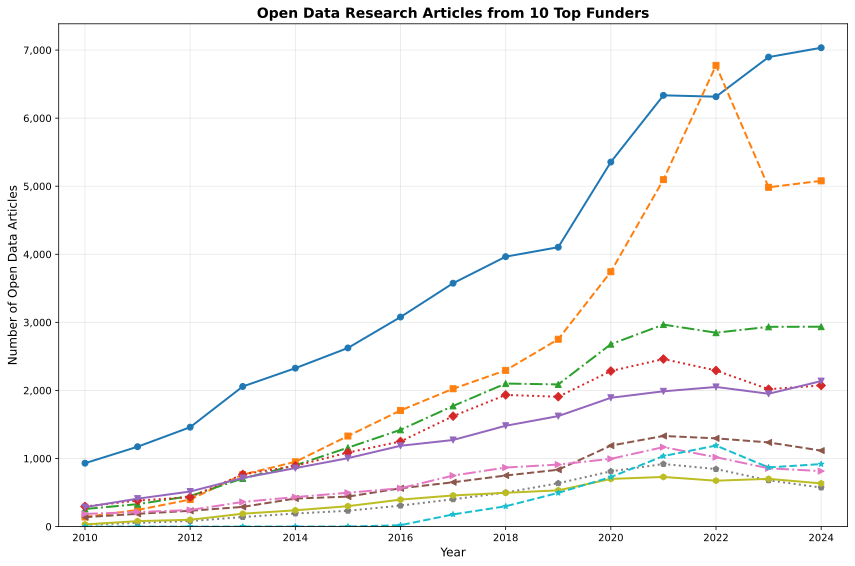
\includegraphics[width=\linewidth]{figures/openss_funder_counts_by_year_v2.png}
            \captionof{figure}{Total number of research articles with open data among 10 biomedical funders 2010--2024.} 
        \end{minipage}\hfill{\color{COL5}\vline}\hfill\begin{minipage}[t]{0.475\linewidth}\centering
            \vspace{0pt}
            \includegraphics[width=\linewidth]{figures/openss_funder_percentages_by_year_v2.png}
            \captionof{figure}{Percentage of research articles with open data among 10 top funders 2010--2024.}
        \end{minipage}\par

        \vspace{2\baselineskip}
        \begingroup
\arrayrulecolor{COL5}
\rowcolors{2}{COL5!10}{white}
\setlength{\tabcolsep}{23.5pt}
\begin{tabular}{llS[table-format=6.0]S[table-format=5.0]S[table-format=2.2,table-align-text-post=false]}
\toprule
\textbf{} & \textbf{}
& \textbf{Research Pubs}
& \textbf{Pubs w/}
& \textbf{\% Pubs w/} \\
\textbf{Funder Name}
& \textbf{Country}
& \textbf{2010--2024}
& \textbf{Data Sharing}
& \textbf{Data Sharing} \\
\midrule
Howard Hughes Medical Institute                                & USA            & \cellcolor{rgb,255:red,198;green,198;blue,255}10189  & 2503  & \cellcolor{rgb,255:red,255;green,153;blue,102}24.6\% \\
United States Department of Agriculture                        & USA            & \cellcolor{rgb,255:red,222;green,222;blue,255}20060  & 4328  & \cellcolor{rgb,255:red,255;green,185;blue,151}21.6\% \\
Department of Biotechnology                                    & India          & \cellcolor{rgb,255:red,198;green,198;blue,255}10188  & 1990  & \cellcolor{rgb,255:red,255;green,208;blue,185}19.5\% \\
Czech Science Foundation                                       & Czech Republic & \cellcolor{rgb,255:red,178;green,178;blue,255}5897   & 1103  & \cellcolor{rgb,255:red,255;green,217;blue,198}18.7\% \\
Department of Energy                                           & USA            & \cellcolor{rgb,255:red,226;green,226;blue,255}22368  & 4011  & \cellcolor{rgb,255:red,255;green,226;blue,211}17.9\% \\
Agence Nationale de la Recherche                               & France         & \cellcolor{rgb,255:red,237;green,237;blue,255}30382  & 5304  & \cellcolor{rgb,255:red,255;green,231;blue,219}17.5\% \\
Max Planck Society                                             & Germany        & \cellcolor{rgb,255:red,197;green,197;blue,255}10143  & 1760  & \cellcolor{rgb,255:red,255;green,232;blue,221}17.4\% \\
Centre National de la Recherche Scientifique                   & France         & \cellcolor{rgb,255:red,206;green,206;blue,255}12729  & 2207  & \cellcolor{rgb,255:red,255;green,232;blue,221}17.3\% \\
Royal Society                                                  & UK             & \cellcolor{rgb,255:red,205;green,205;blue,255}12652  & 1929  & \cellcolor{rgb,255:red,254;green,254;blue,255}15.2\% \\
Wellcome Trust                                                 & UK             & \cellcolor{rgb,255:red,255;green,240;blue,232}68683  & 9873  & \cellcolor{rgb,255:red,247;green,247;blue,255}14.4\% \\
Associazione Italiana per la Ricerca sul Cancro                & Italy          & \cellcolor{rgb,255:red,187;green,187;blue,255}7641   & 1080  & \cellcolor{rgb,255:red,245;green,245;blue,255}14.1\% \\
Swiss National Science Foundation                              & Switzerland    & \cellcolor{rgb,255:red,229;green,229;blue,255}24562  & 3431  & \cellcolor{rgb,255:red,244;green,244;blue,255}14.0\% \\
Research Foundation Flanders                                   & Belgium        & \cellcolor{rgb,255:red,196;green,196;blue,255}9776   & 1344  & \cellcolor{rgb,255:red,242;green,242;blue,255}13.8\% \\
National Science Foundation                                    & USA            & \cellcolor{rgb,255:red,255;green,205;blue,181}141132 & 19368 & \cellcolor{rgb,255:red,241;green,241;blue,255}13.7\% \\
Natural Sciences and Engineering Research Council of Canada    & Canada         & \cellcolor{rgb,255:red,234;green,234;blue,255}28642  & 3895  & \cellcolor{rgb,255:red,240;green,240;blue,255}13.6\% \\
Australian Research Council                                    & Australia      & \cellcolor{rgb,255:red,231;green,231;blue,255}26111  & 3511  & \cellcolor{rgb,255:red,239;green,239;blue,255}13.4\% \\
National Institutes of Health                                  & USA            & \cellcolor{rgb,255:red,255;green,153;blue,102}426267 & 57220 & \cellcolor{rgb,255:red,239;green,239;blue,255}13.4\% \\
Austrian Science Fund                                          & Austria        & \cellcolor{rgb,255:red,212;green,212;blue,255}15381  & 2014  & \cellcolor{rgb,255:red,236;green,236;blue,255}13.1\% \\
European Commission                                            & EU             & \cellcolor{rgb,255:red,255;green,189;blue,157}196678 & 25542 & \cellcolor{rgb,255:red,235;green,235;blue,255}13.0\% \\
Deutsche Forschungsgemeinschaft                                & Germany        & \cellcolor{rgb,255:red,255;green,231;blue,219}82116  & 10660 & \cellcolor{rgb,255:red,235;green,235;blue,255}13.0\% \\
Russian Science Foundation                                     & Russia         & \cellcolor{rgb,255:red,203;green,203;blue,255}11734  & 1506  & \cellcolor{rgb,255:red,234;green,234;blue,255}12.8\% \\
Netherlands Organisation for Scientific Research               & Netherlands    & \cellcolor{rgb,255:red,216;green,216;blue,255}17223  & 2149  & \cellcolor{rgb,255:red,231;green,231;blue,255}12.5\% \\
Japan Agency for Medical Research and Development              & Japan          & \cellcolor{rgb,255:red,212;green,212;blue,255}15385  & 1872  & \cellcolor{rgb,255:red,229;green,229;blue,255}12.2\% \\
UK Research and Innovation                                     & UK             & \cellcolor{rgb,255:red,255;green,194;blue,163}179659 & 21694 & \cellcolor{rgb,255:red,228;green,228;blue,255}12.1\% \\
Ministerio de Economia y Competitividad                        & Spain          & \cellcolor{rgb,255:red,235;green,235;blue,255}29285  & 3490  & \cellcolor{rgb,255:red,227;green,227;blue,255}11.9\% \\
Swedish Research Council                                       & Sweden         & \cellcolor{rgb,255:red,235;green,235;blue,255}29409  & 3486  & \cellcolor{rgb,255:red,226;green,226;blue,255}11.8\% \\
Fundacao de Amparo a Pesquisa do Estado de Sao Paulo           & Brazil         & \cellcolor{rgb,255:red,221;green,221;blue,255}19810  & 2335  & \cellcolor{rgb,255:red,226;green,226;blue,255}11.8\% \\
National Key Research and Development Program                  & China          & \cellcolor{rgb,255:red,254;green,254;blue,255}48760  & 5732  & \cellcolor{rgb,255:red,225;green,225;blue,255}11.8\% \\
Bundesministerium für Bildung und Forschung                    & Germany        & \cellcolor{rgb,255:red,232;green,232;blue,255}26596  & 3091  & \cellcolor{rgb,255:red,224;green,224;blue,255}11.6\% \\
Ministry of Education, Culture, Sports, Science and Technology & Japan          & \cellcolor{rgb,255:red,234;green,234;blue,255}28406  & 3270  & \cellcolor{rgb,255:red,223;green,223;blue,255}11.5\% \\
China Scholarship Council                                      & China          & \cellcolor{rgb,255:red,211;green,211;blue,255}15005  & 1708  & \cellcolor{rgb,255:red,222;green,222;blue,255}11.4\% \\
European Regional Development Fund                             & EU             & \cellcolor{rgb,255:red,255;green,249;blue,246}56374  & 6396  & \cellcolor{rgb,255:red,222;green,222;blue,255}11.3\% \\
Japan Science and Technology Agency                            & Japan          & \cellcolor{rgb,255:red,209;green,209;blue,255}13996  & 1570  & \cellcolor{rgb,255:red,221;green,221;blue,255}11.2\% \\
Fundacao para a Ciencia e a Tecnologia                         & Portugal       & \cellcolor{rgb,255:red,216;green,216;blue,255}17108  & 1844  & \cellcolor{rgb,255:red,217;green,217;blue,255}10.8\% \\
National Science Centre                                        & Poland         & \cellcolor{rgb,255:red,210;green,210;blue,255}14256  & 1528  & \cellcolor{rgb,255:red,217;green,217;blue,255}10.7\% \\
American Heart Association                                     & USA            & \cellcolor{rgb,255:red,202;green,202;blue,255}11428  & 1204  & \cellcolor{rgb,255:red,215;green,215;blue,255}10.5\% \\
Coordenacao de Aperfeicoamento de Pessoal de Nivel Superior    & Brazil         & \cellcolor{rgb,255:red,236;green,236;blue,255}29668  & 3123  & \cellcolor{rgb,255:red,215;green,215;blue,255}10.5\% \\
Italian Ministry                                               & Italy          & \cellcolor{rgb,255:red,220;green,220;blue,255}19005  & 1947  & \cellcolor{rgb,255:red,213;green,213;blue,255}10.2\% \\
Japan Society for the Promotion of Science                     & Japan          & \cellcolor{rgb,255:red,255;green,241;blue,235}66236  & 6258  & \cellcolor{rgb,255:red,206;green,206;blue,255}9.4\% \\
China Postdoctoral Science Foundation                          & China          & \cellcolor{rgb,255:red,229;green,229;blue,255}24691  & 2328  & \cellcolor{rgb,255:red,206;green,206;blue,255}9.4\% \\
National Natural Science Foundation of China                   & China          & \cellcolor{rgb,255:red,255;green,153;blue,102}420824 & 38274 & \cellcolor{rgb,255:red,203;green,203;blue,255}9.1\% \\
Bill and Melinda Gates Foundation                              & USA            & \cellcolor{rgb,255:red,226;green,226;blue,255}22670  & 2046  & \cellcolor{rgb,255:red,203;green,203;blue,255}9.0\% \\
Ministry of Science and Technology                             & Taiwan         & \cellcolor{rgb,255:red,255;green,248;blue,244}57698  & 5186  & \cellcolor{rgb,255:red,202;green,202;blue,255}9.0\% \\
National Health and Medical Research Council                   & Australia      & \cellcolor{rgb,255:red,237;green,237;blue,255}30425  & 2667  & \cellcolor{rgb,255:red,201;green,201;blue,255}8.8\% \\
Canadian Institutes of Health Research                         & Canada         & \cellcolor{rgb,255:red,242;green,242;blue,255}35617  & 2908  & \cellcolor{rgb,255:red,196;green,196;blue,255}8.2\% \\
National Research Foundation of Korea                          & Korea          & \cellcolor{rgb,255:red,255;green,230;blue,218}84068  & 5625  & \cellcolor{rgb,255:red,183;green,183;blue,255}6.7\% \\
National Institute for Health Research                         & UK             & \cellcolor{rgb,255:red,253;green,253;blue,255}47528  & 2865  & \cellcolor{rgb,255:red,178;green,178;blue,255}6.0\% \\
\bottomrule
\end{tabular}
\arrayrulecolor{black}
\endgroup
        
       
        
        
        \begin{minipage}{0.6\linewidth}\raggedright
            
        \end{minipage}\hfill
    }

    
\end{poster}
\end{document}